\documentclass[11pt]{aghdpl}
% \documentclass[en,11pt]{aghdpl}  % praca w języku angielskim

% Lista wszystkich języków stanowiących języki pozycji bibliograficznych użytych w pracy.
% (Zgodnie z zasadami tworzenia bibliografii każda pozycja powinna zostać utworzona zgodnie z zasadami języka, w którym dana publikacja została napisana.)
\usepackage[english,polish]{babel}

% Użyj polskiego łamania wyrazów (zamiast domyślnego angielskiego).
\usepackage{polski}

\usepackage[utf8]{inputenc}

% dodatkowe pakiety

\usepackage{mathtools}
\usepackage{amsfonts}
\usepackage{amsmath}
\usepackage{amsthm}

% --- < bibliografia > ---

\usepackage[
style=numeric,
sorting=none,
%
% Zastosuj styl wpisu bibliograficznego właściwy językowi publikacji.
language=autobib,
autolang=other,
% Zapisuj datę dostępu do strony WWW w formacie RRRR-MM-DD.
urldate=iso8601,
% Nie dodawaj numerów stron, na których występuje cytowanie.
backref=false,
% Podawaj ISBN.
isbn=true,
% Nie podawaj URL-i, o ile nie jest to konieczne.
url=false,
%
% Ustawienia związane z polskimi normami dla bibliografii.
maxbibnames=3,
% Jeżeli używamy BibTeXa:
backend=bibtex
]{biblatex}

\usepackage{csquotes}
% Ponieważ `csquotes` nie posiada polskiego stylu, można skorzystać z mocno zbliżonego stylu chorwackiego.
\DeclareQuoteAlias{croatian}{polish}

\addbibresource{bibliografia.bib}

% Nie wyświetlaj wybranych pól.
%\AtEveryBibitem{\clearfield{note}}


% ------------------------
% --- < listingi > ---

% Użyj czcionki kroju Courier.
\usepackage{courier}

\usepackage{listings}
\lstloadlanguages{TeX}

\lstset{
	literate={ą}{{\k{a}}}1
           {ć}{{\'c}}1
           {ę}{{\k{e}}}1
           {ó}{{\'o}}1
           {ń}{{\'n}}1
           {ł}{{\l{}}}1
           {ś}{{\'s}}1
           {ź}{{\'z}}1
           {ż}{{\.z}}1
           {Ą}{{\k{A}}}1
           {Ć}{{\'C}}1
           {Ę}{{\k{E}}}1
           {Ó}{{\'O}}1
           {Ń}{{\'N}}1
           {Ł}{{\L{}}}1
           {Ś}{{\'S}}1
           {Ź}{{\'Z}}1
           {Ż}{{\.Z}}1,
	basicstyle=\footnotesize\ttfamily,
}

% ------------------------

\AtBeginDocument{
	\renewcommand{\tablename}{Tabela}
	\renewcommand{\figurename}{Rys.}
}

% ------------------------
% --- < tabele > ---

\usepackage{array}
\usepackage{tabularx}
\usepackage{multirow}
\usepackage{booktabs}
\usepackage{makecell}
\usepackage{float}
\usepackage[flushleft]{threeparttable}

% defines the X column to use m (\parbox[c]) instead of p (`parbox[t]`)
\newcolumntype{C}[1]{>{\hsize=#1\hsize\centering\arraybackslash}X}


%---------------------------------------------------------------------------

\author{Adrian Moskwik}
\shortauthor{A. Moskwik}

%\titlePL{Przygotowanie bardzo długiej i pasjonującej pracy dyplomowej w~systemie~\LaTeX}
%\titleEN{Preparation of a very long and fascinating bachelor or master thesis in \LaTeX}

\titlePL{Opracowanie, konstrukcja oraz uruchomienie robota mobilnego, kołowego z napędem różnicowym}
\titleEN{Development, construction and commissioning of mobile, wheeled robot with differential drive}


\shorttitlePL{Opracowanie, konstrukcja oraz uruchomienie robota mobilnego, kołowego z napędem różnicowym} % skrócona wersja tytułu jeśli jest bardzo długi
\shorttitleEN{Development, construction and commissioning of mobile, wheeled robot with differential drive}

\thesistype{Projekt dyplomowy}
%\thesistype{Master of Science Thesis}

\supervisor{dr inż. Łukasz Więckowski}
%\supervisor{Marcin Szpyrka PhD, DSc}

\degreeprogramme{Automatyka i Robotyka}
%\degreeprogramme{Computer Science}

\date{2020}

\department{Katedra Automatyki i Robotyki}
%\department{Department of Applied Computer Science}

\faculty{Wydział Elektrotechniki, Automatyki,\protect\\[-1mm] Informatyki i Inżynierii Biomedycznej}
%\faculty{Faculty of Electrical Engineering, Automatics, Computer Science and Biomedical Engineering}

\acknowledgements{Serdecznie dziękuję \dots tu ciąg dalszych podziękowań np. dla promotora, żony, sąsiada itp.}


\setlength{\cftsecnumwidth}{10mm}

%---------------------------------------------------------------------------
\setcounter{secnumdepth}{4}
\brokenpenalty=10000\relax

\begin{document}

\titlepages

% Ponowne zdefiniowanie stylu `plain`, aby usunąć numer strony z pierwszej strony spisu treści i poszczególnych rozdziałów.
\fancypagestyle{plain}
{
	% Usuń nagłówek i stopkę
	\fancyhf{}
	% Usuń linie.
	\renewcommand{\headrulewidth}{0pt}
	\renewcommand{\footrulewidth}{0pt}
}

\setcounter{tocdepth}{2}
\tableofcontents

\clearpage
\chapter{Wspęp}


Żaneta dzban 


Robotyka jest gałęzią technologii zajmującą się projektowaniem, budową, sterowaniem i użytkowaniem robotów. 

\section{Cel i założenia pracy}

Celem projektu dyplomowego było zaprojektowanie, zbudowanie oraz uruchomienie platformy dydaktycznej robota mobilnego, kołowego o napędzie elektrycznym, różnicowym. Napędy robota zostały zrealizowane za pomocą czterech silników DC, wraz z dedykowanym układem mocy Pololu VNH5019, posiadającym własny mikro kontroler oraz jednostkę inercyjną. Robot mobilny został wyposażony w sterownik główny typu: Intel Up-Board, wraz z dedykowanym systemem wizyjnym Intel RealSense R200. Sterownik robota został oprogramowany w jęzuku C/C++, był on odpowiedzialny za sterowanie napędami, czyli zadawanie oraz stabilizację prędkości, a także wyliczanie akualnej pozycj oraz parametrów ruchu na podstawie odczytow z enkoderów oraz jednostki inercyjnej. Informacje z platformy zostały udostępnione dla systemu nadrzędnego, pracującego pod kontrolą systmeu operacyjnego, wykrzystującego komunikację między wątkową ROS. Testy działania robota mobilnego zostały przeprowadzone z wykorzystaniem dedykowanych w robotyce mobilnej narzędzi programowych tj: ROS/RViz, Gazebo, MATLAB Robotics System Toolbox.

\section{Układ pracy}

Projekt dyplomowy składa się z sześciu rozdziałów. Rozdział pierwszy został poświęcony wprowadzeniu w tematykę robotyki oraz określeniu celów przed rozpoczęciem pracy nad projektem. W rozdziale drugim przybliżona została tematyka robotów mobilnych, komunikacja między wątkowa oraz platforma dydaktyczna Tutrlebot. W rozdziale trzecim został przedstawiona konstrukcja robota oraz charakterystyka podzespołów wykorzystanych do jego konstrukcji. Rozdział czwarty został poświęcony oprogramowaniu sterownika robota. W rozdziale piątym zostało opisane zastosowanie komunikacji między wątkowej. Rozdział szósty jest poświęcony testom działania robota mobilnego.

\chapter{Wprowadzenie teoretyczne}

\section{Roboty mobilne}

Robot mobilny to autonomiczny pojazd zdolny do poruszania się po swoim środowisku, bez fizycznego przywiązania do jednej lokalizacji \cite{mobile_robot}. Oznacza to, że ich przestrzeń robocza jest konstrukcyjnie nieograniczona, nie posiada ograniczeń takich jak np. przewodowy sterujące podłączone stacjonarnie do jednego miejsca. Dodatkowo nie wymagają one bezpośredniej ingerencji człowieka. Sprawia to, że ich konstrukcja mechaniczna może przyjmować dowolne rozmiary potrzebne do wykonywanych zadań, bez ograniczeń związanych z czynnikiem ludzkim. 

Środowiskiem robota mobilnego może być ląd, woda lub powietrze. W oparciu o środowisko poruszania się, roboty mobilne można podzielić na:

\begin{itemize}
\item
 \textit{Jeżdżące}
 \item
 \textit{Kroczące}
 \item 
 \textit{Pływające}
 \item 
 \textit{Latające} 
 \item 
 \textit{Inne}
\end{itemize}

 Najbardziej popularną grupą są roboty jeżdżące. Grupa ta rozwija się w szybkim tempie, jest to spowodowane między innymi inwestycjami globalnych koncernów motoryzacyjnych. Skupiają się one na rozwoju technologicznym i dążą do coraz większej autonomiczności swoich pojazdów. Prekursorem w tej dziedzinie jest firma Tesla, która zapowiedziała, że  w połowie 2020 roku, w ich pojazdach zostanie wprowadzony tryb pełnej autonomicznej jazdy. 
 
 Ze względu na dynamiczny rozwój tej grupy robotów mobilnych, są one też popularne pośród konstruktorów-amatorów, którzy zajmują się budową robotów w celach dydaktycznych, badawczych lub hobbistycznych.  
\section{Napęd różnicowy}

 Napęd różnicowy umożliwia kołom na jednej osi uzyskanie różnych prędkości obrotowych, jest to niezbędne w przypadku robotów o napędzie kołowym bez skrętnej osi. Podczas ruchu po łuku, koła pojazdu pokonują inną drogę. Zastosowanie napędu różnicowego pozwala, aby toczyły się one po swoich torach ruchu bez poślizgu, osiągając różne prędkości obrotowe.
\section{Robot Operating System}

ROS(Robot Operating System) jest to meta-operacyjny systemem dla robotów, który posiada otwarty dostęp do kodu źródłowego. Podobnie jak zwyczajny system operacyjny zapewnia warstwę abstrakcji sprzętowej, kontrolę urządzeń niskopoziomowych, implementacje powszechnie używanych funkcjonalności \cite{ROS}. ROS różni się jednak od powszechnego systemu, możliwością komunikacji między wątkowej. Procesy mogą komunikować się ze sobą w czasie swojego wykonywania. Sprawia to, że ROS jest dobrym systemem do wsparcia sterowania robotem oraz czujnikami(Rys.\ref{fig:ROS_meta_system}). Kolejną zaletą systemu ROS jest możliwość współpracy z większością popularnych systemów operacyjnych takich jak Windows, Linux, Mac, Android lub iOS. 

\begin{figure}[ht]
	\centering
	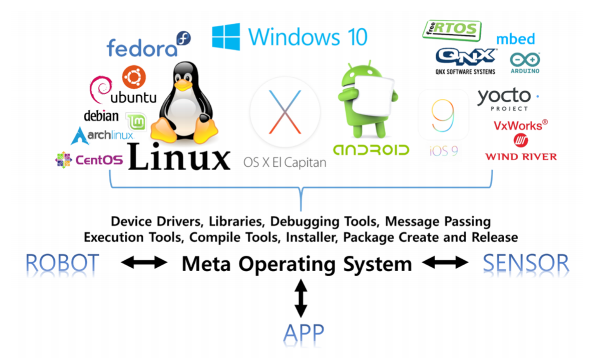
\includegraphics[scale=1]{ROS_meta_system.png}
	\caption{ROS jako meta-operacyjny system \cite{ROS}.}
	\label{fig:ROS_meta_system}
\end{figure}

Główne założenia sytemu ROS można przedstawić jako \cite{ROS_goals}:

\begin{itemize}
	\item 
	\textit{Komunikacja P2P(peer to peer)} - model komunikacji w sieci komputerowej zapewniający wszystkim hostom te same uprawnienia \cite{P2P}.
	\item
	\textit{Oparty na narzędziach} - duża liczba małych narzędzi jest używana do budowania i uruchamiania różnych komponentów systemu.
	\item 
	\textit{Wielojęzykowy} - wspiera wiele języków programowania.
	\item 
	\textit{Niezagnieżdżony} - tworzenie tylko małych plików wykonywalnych, które ujawniają bibliotekę funkcjonalności do systemu ROS. Pozwala to na łatwiejszą ekstrakcję kodu i użycie go ponownie poza pierwotnym przeznaczeniem.  
	\item 
	\textit{Darmowy i posiadający otwarty dostęp do kodu źródłowego.}
\end{itemize}

\begin{figure}[ht]
	\centering
	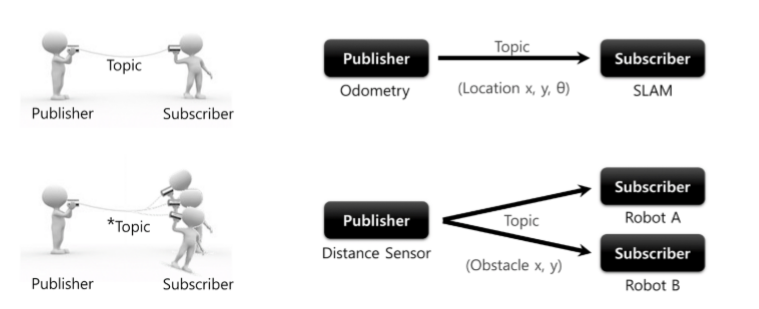
\includegraphics[scale=0.8]{topic.png}
	\caption{Komunikacja z wykorzystaniem tematów. \cite{ROS}.}
	\label{fig:topic}
\end{figure}

Komunikacja odbywa się między \textit{węzłami(ang. nodes)}, czyli pojedynczymi procesami działającymi w ramach systemu ROS. Kanał komunikacyjny między węzłami to \textit{temat(ang. topic)}. \textit{Wiadomość(ang message)} to dane wysyłane między węzłami za pomocą tematu. Węzeł publikuje lub subskrybuje temat, czyli wysyła lub pobiera z niego wiadomość. Schemat komunikacji przy pomocy tematów został przedstawiony na Rys.\ref{fig:topic}.




\section{TurtleBot}

Turtlebot jest standardowym robotem platformowym wykorzystującym komunikację między wątkową ROS. Platforma ta jest bardzo popularna wśród deweloperów, a także studentów, ponieważ doskonale nadaje się do celów dydaktycznych. Oprogramowanie posiada otwarty dostęp do kodu źródłowego \cite{turtlebot3}. Upraszcza to zrozumienie zasady działania platformy, ponieważ umożliwia łatwy dostęp do dokumentacji, w której znajduje się opis działania poszczególnych modułów. 

\begin{figure}[ht]
	\centering
	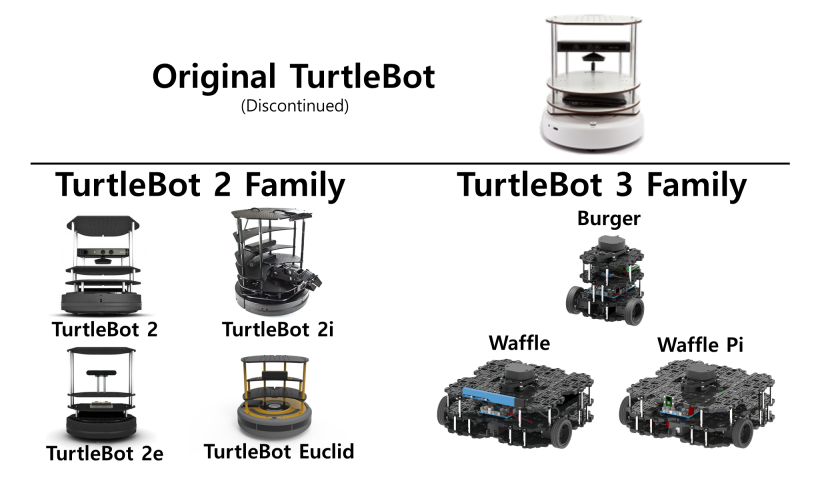
\includegraphics[scale=0.7]{turtlebot.png}
	\caption{Rodzina robotów TurtleBot. \cite{turtlebot}.}
	\label{fig:turtlebot}
\end{figure}  

Istnieją trzy wersje robotów serii TurtleBot(Rys.\ref{fig:turtlebot}). Najnowsza z nich została zaprezentowana w maju 2017 roku. TurtleBot3 jest małym, niskobudżetowym, programowalnym, opartym na komunikacji między wątkowej ROS robotem mobilnym, który służy do celów edukacyjnych, badawczych lub hobbistycznych.  Składa się on z wewnętrznego komputera, mikro kontrolera, systemu wizyjnego i czujników.  Wewnętrzny komputer komunikuje się przy pomocy komunikacji ROS przez WiFi ze zdalnym komputerem. Udostępnia on dane z czujników i otrzymuje sterowanie, czyli prędkość liniową i kątową, która jest następnie przeliczana na wartość prędkości obrotowej każdego z kół. Mikro kontroler komunikuje się z komputerem wewnętrznym przy pomocy szeregowej komunikacji między wątkowej. 



\chapter{Konstrukcja robota}

Do konstrukcji robota została zakupiona platforma \textit{4WD Outdoor Mobile Platform}. Składa się ona metalowej obudowy oraz czterech silników i kół \cite{Outdoor_robot}. Posiada ona poziomowy charakter budowy, jednakże konstruowany robot składa się tylko z dolnego poziomu. 

Głównym założeniem mechanicznym jest stworzenie jeżdżącego robota mobilnego poruszającego się po środowisku lądowym. Ruch robota jest możliwy zarówno po płaskiej i nierównej powierzchni. Podzespoły robota można podzielić na  układ napędowy, układ sterujący, czujniki oraz zasilanie.



\section{Komunikacja podzespołów}

Sposób komunikacji podzespołów został przedstawiony na Rys. \ref{fig:schemat}. 

Jednostka mocy Pololu Dual VNH5019 jest dwukanałowa. Oznacza to, że możliwe jest sterowanie prędkością po dwóch stronach robota, a nie na każdym kole. Silniki po tej samej stronie zostały połączone szeregowo, a następnie trwale połączone z  jednostką mocy, która z kolei została połączona z mikro kontrolerem. 

Napięcie znamionowe dla STM32L476RG  wynosi od 1.71 do 3.6V, natomiast napięcie sygnałów A i B pochodzących od enkoderów przyjmuje wartość 5V. W tym celu został wykorzystany konwerter poziomów, który zmniejszył ich napięcie do 3.3V, które jest bezpieczne dla użytego mikro kontrolera.

Z mikro kontrolerem łączy się dodatkowo, poprzez komunikacje I2C, jednostka inercyjna MPU9250. STM32 komunikuje się poprzez port szeregowy z głównym sterownikiem. Up Board otrzymuje ponadto dane z dedykowanego systemu wizyjnego, połączonego poprzez USB 3.0 OTG i lidaru połączonego poprzez USB 2.0. Dodatkowo na zewnątrz urządzenia został wyprowadzony Qilive Hub z 4 portami USB 2.0. Pozwali to na rozbudowanie robota o kolejne moduły bez konieczności ingerencji elektronikę znajdującą się wewnątrz obudowy.

Główny sterownik wymienia informacje ze zdalnym komputerem poprzez wi-fi. Wykorzystany do tego został zdalny moduł wi-fi ASUS WL-167g, jest on połączony z główny sterownikiem poprzez USB 2.0.

\begin{figure}[!ht]
	\centering
	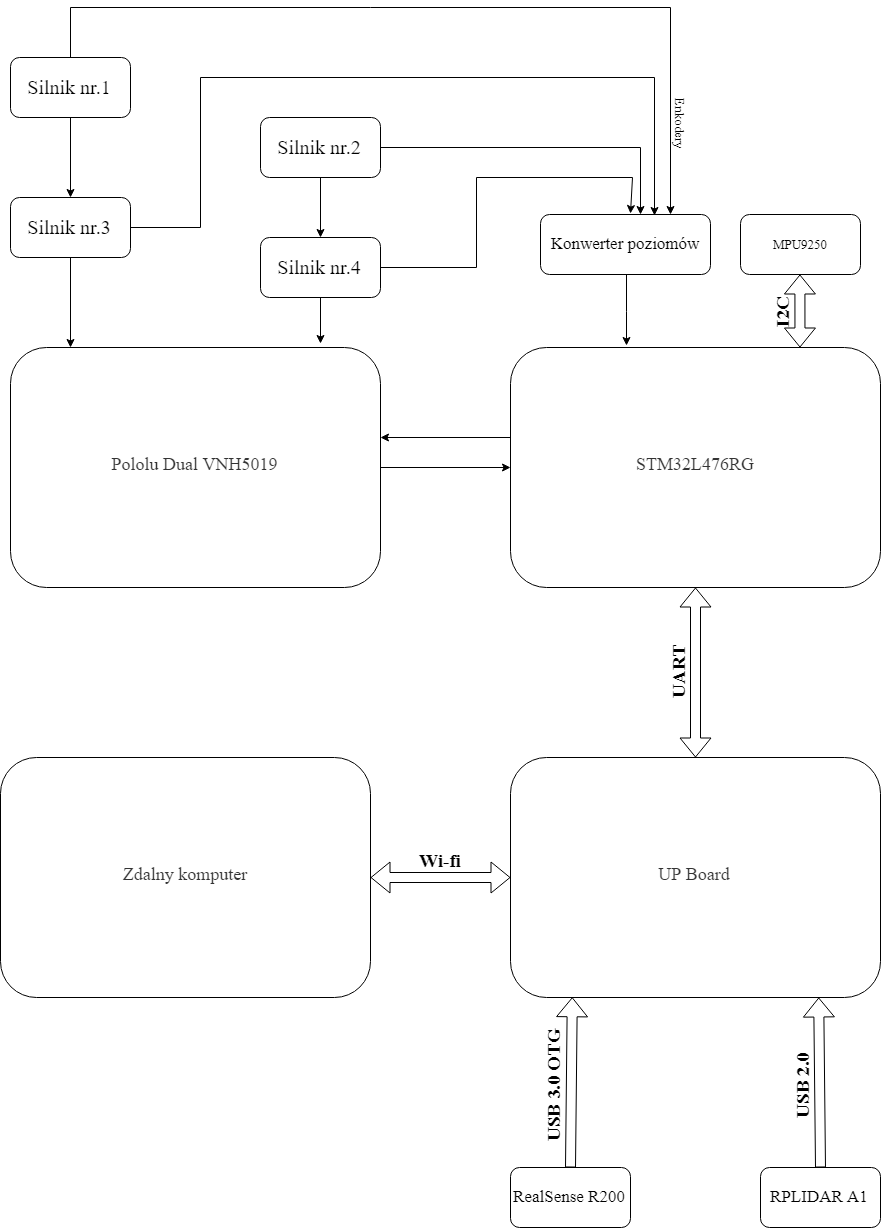
\includegraphics[scale=0.5]{schemat.png}
	\caption{Schemat komunikacji podzespołów.}
	\label{fig:schemat}
\end{figure}


\section{Układ napędowy}
Elementami wykonawczymi robota są części napędowe, czyli silniki DC. Nadają one kołom prędkość obrotową zadaną sterowaniem otrzymanym z układu sterującego. Wykorzystane silniki są dedykowanymi elementami do wykorzystanej obudowy robota.
\subsection{Silniki prądu stałego}

Napęd robota stanowią 4 silniki prądu stałego zintegrowane z przekładnią zębatą  i połączone z enkoderami kwadratowymi (Rys.\ref{fig:silnik}). Oznaczenie modelu to No.GB37Y3530-12V-251R. Przełożenie przekładni wynosi 43,8:1. Enkoder kwadratowy zapewnia rozdzielczość 16 pomiarów na obrót wału silnika co odpowiada 700 pomiarom na obrót wału wyjściowego. Oznacza to, że impuls będzie występował co 0.6mm przebytej drogi. Najważniejsze dane techniczne silnika zostały przedstawione w tabeli \ref{parametry_silnika}.


\begin{figure}[ht]
	\centering
	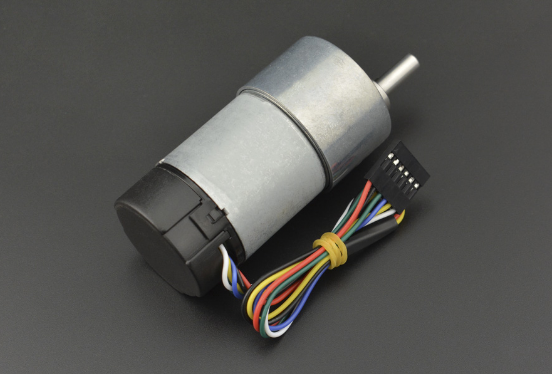
\includegraphics[scale=0.7]{silnik.png}
	\caption{Silnik DC serii Gear Motor.}
	\label{fig:silnik}
\end{figure}



\begin{table}[]
	\centering
	\caption{Parametry silnika.}
	\label{parametry_silnika}
	\begin{tabular}{|c|c|}
		\hline
		\multicolumn{2}{|c|}{\textbf{Specyfikacja}} \\ \hline
		Napięcie zasilania                & 1 - 12V \\ \hline
		Natężenie prądu bez obciążenia    & 350mA   \\ \hline
		Prędkość obrotowa bez obciążenia  & 251RPM  \\ \hline
		Napięcie znamionowe enkodera      & 5V      \\ \hline
		Typ enkodera                      & Hall    \\ \hline
		Waga                              & 205g    \\ \hline
	\end{tabular}
\end{table}

\subsection{Koła}

Do poruszania się robota zostały wykorzystane koła o średnicy \i134mm i szerokości 48mm z gumową oponą terenową(Rys. \ref{fig:koła}). Szeroka opona zapewnia  większą powierzchnię styku z podłożem. Skutkuje to uzyskaniem lepszej przyczepności oraz skróceniem drogi hamowania w stosunku do węższej opony.
\begin{figure}[ht]
	\centering
	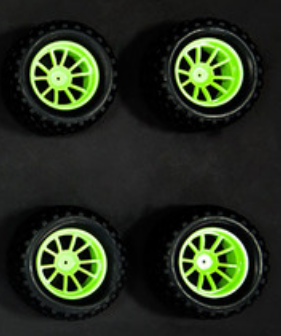
\includegraphics[scale=0.8]{koła.png}
	\caption{Koła robota.}
	\label{fig:koła}
\end{figure}

Dobrane silniki i koła pozwalają robotowi mobilnemu na uzyskanie maksymalnej prędkości równej ok. 1.5$\frac{m}{s}$. Osiągana prędkość jest wystarczająca do planowanych zastosowań robot.

\section{Układ sterujący}

Układ sterujący ma na celu wyznaczenie i zadanie sterowania na elementy wykonawcze. W tym przypadku będzie to zadawanie  prędkości obrotowej na koła, poprzez zmianę wartości natężenia prądu podawanego na silniki.  Wykorzystany w tym celu został dwukanałowy układ mocy, mikro kontroler oraz nadrzędny sterownik główny. Na zdalnym komputerze jest wyliczana prędkości liniowa i kątowa, którą ma osiągnąć robot. Informację tę pobiera mikro kontroler i na jej podstawie przelicza prędkość z jaką mają się poruszać prawe i lewe koła. Następnie przy pomocy układu mocy prąd o odpowiednim natężeniu jest podawany na silniki. 


\subsection{Układ mocy}

Do sterowania napędami zastosowany został układ mocy Pololu Dual VNH5019 Motor Driver Shield (Rys.\ref{fig:pololu}). Układ ten jest kompatybilny z platformą Arduino. Posiada własną bibliotekę, która pozwala w bardzo prostu sposób sterować silnikami prądu stałego zasilane napięciem z zakresu 5.5 - 24V o ciągłym poborze prądu do 12A.  Posiada dwa kanały do sterowania silnikami, do każdego kanału zostały wpięte dwa silniki znajdujące się po tej samej stronie, połączone w sposób równoległy.   

Układ umożliwia zmianę kierunku obrotów silnika oraz regulacje prędkości obrotowej poprzez sygnał PWM. Działanie poszczególnych pinów zostało przedstawione w Tabeli \ref{pololu_pins}.

\begin{figure}[ht]
	\centering
	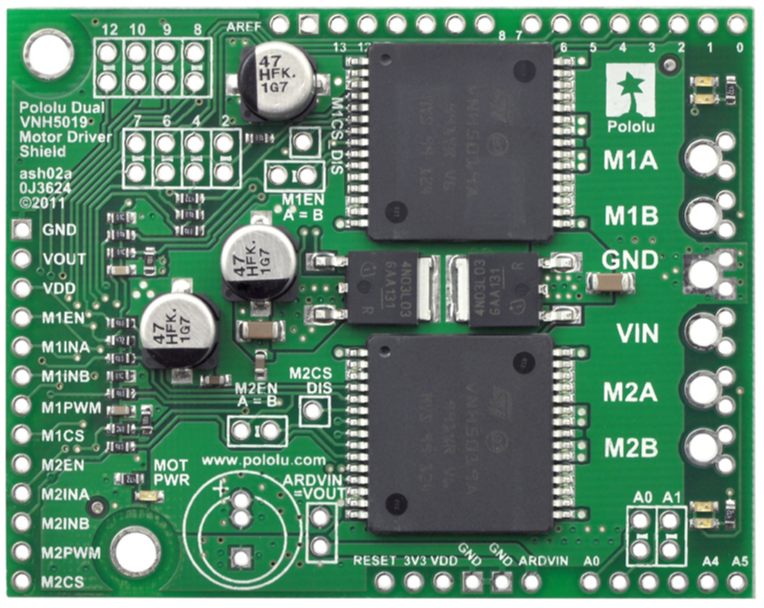
\includegraphics[scale=0.6]{pololu.png}
	\caption{Pololu Dual VNH5019 Motor Driver Shield.}
	\label{fig:pololu}
\end{figure}



\begin{table}[!h]
	\centering
	\caption{Piny sterownika silników.}
	\label{pololu_pins}
	\begin{tabular}{|c|c|}
		\hline
		\textbf{VNH5019 Pin} & \textbf{Zastosowanie}           \\ \hline
		M1INA                & Kierunek silnika 1 - wejście A  \\ \hline
		M1INB                & Kierunek silnika 1 - wejście B  \\ \hline
		M1EN/DIAG            & Silnik 1 – informacja o błędzie \\ \hline
		M2INA                & Kierunek silnika 2 – wejście A  \\ \hline
		M2INB                & Kierunek silnika 2 – wejście B  \\ \hline
		M1PWM                & Sterowanie prędkością silnika 1 \\ \hline
		M2PWM                & Sterowanie prędkością silnika 2 \\ \hline
		M2EN/DIAG            & Silnik 2 – informacja o błędzie \\ \hline
		M1CS                 & Odczyt prądu na silniku 1       \\ \hline
		M2CS                 & Odczyt prądu na silniku 2       \\ \hline
	\end{tabular}
\end{table}




\subsection{Mikrokontroler}


Do sterowania robotem wykorzystany został mikro kontroler  STM32 Nucleo-L476RG(Rys.\ref{fig:stm32}) z wydajnym rdzeniem Arm® Cortex®-M4 32-bit RISC, taktującym do 80Mhz. Wyposażony jest w 1MB pamięci flash oraz 128KB pamięci SRAM. Obsługuje interfejsy komunikacyjne takie jak SPI, I2C, USART, UART, USB, CAN. Posiada wbudowany programator i debugger ST-LINK/V2-1. Pozwala na prace w trybie kompatybilności z Arduino Uno, pozwala to wykorzystywać do jego programowania środowiska dedykowane językowi Arduino. Umożliwia obsługę szesnastu liczników różnorakiego zastosowania. Posiada 51pinów typu GPIO(\textit{general-purpose input/output}), a także 16 linii przerwań zewnętrznych. Źródłem zasilania jest przez port USB z napięciem między 3.0-3.6V.

\begin{figure}[ht]
	\centering
	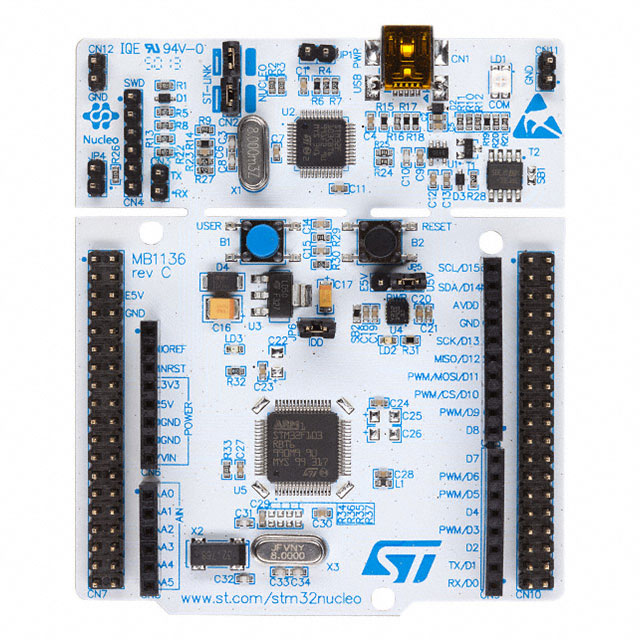
\includegraphics[scale=0.40]{stm32.png}
	\caption{Mikrokontroler STM32 Nucleo-L476RG.}
	\label{fig:stm32}
\end{figure}

Zastosowany mikro kontroler pozwolił na integrację z jednostką mocy, ponieważ jego budowa umożliwia pracę w trybie kompatybilnym z Arduino Uno. Wykorzystany STM pozwala więc na wykorzystanie bibliotek dostępnych dla Arduino, ale dodatkowo oferuje większą pamięć podręczną i moc obliczeniową. Znaczącą zaletą jest także duża liczba pinów GPIO. Zostały one wykorzystane do uzyskania komunikacji z enkoderami, jednostką inercyjną, a także jednostką mocy. 

W dokumentacji technicznej mikro kontrolera zostały odnalezione piny odpowiedzialne za poszczególne funkcje, a następnie stworzono schemat wszystkich potrzebnych połączeń(Tabela. \ref{stm_pins}). Połączenia związane z enkoderami i jednostką inercyjną zostały trwale wykonane na płytce prototypowej do lutowania, natomiast piny związane z jednostką mocy posiadają możliwość wyjęcia.  

% Please add the following required packages to your document preamble:
% \usepackage{graphicx}
\begin{table}[ht]
	\centering
	\caption{Połączenia pinów STM32 Nucleo-L476RG. }
	\label{stm_pins}
	\begin{tabular}{|c|c|}
		\hline
		\textbf{STM32 Pin} & \textbf{Zastosowanie} \\ \hline
		PA10               & VNH5019  - M1INA      \\ \hline
		PB5                & VNH5019 - M1INB       \\ \hline
		PB10               & VNH5019 - M1EN/DIAG   \\ \hline
		PA8                & VNH5019 - M2INA       \\ \hline
		PA9                & VNH5019 - M2INB       \\ \hline
		PC7                & VNH5019 - M1PWM       \\ \hline
		PB6                & VNH5019 - M2PWM       \\ \hline
		PA6                & VNH5019 - M2EN/DIAG   \\ \hline
		PA0                & VNH5019 - M1CS        \\ \hline
		PA1                & VNH5019 - M2CS        \\ \hline
		PB13               & MPU9250 - SCL         \\ \hline
		PB14               & MPU9250 - SDA         \\ \hline
		PC8                & Enkoder 1 - Sygnał A  \\ \hline
		PC6                & Enkoder 1 - Sygnał B  \\ \hline
		PC5                & Enkoder 2 - Sygnał A  \\ \hline
		PA12               & Enkoder 2 - Sygnał B  \\ \hline
		PB2                & Enkoder 3 - Sygnał A  \\ \hline
		PB1                & Enkoder 3 - Sygnał B  \\ \hline
		PB15               & Enkoder 4 - Sygnał A  \\ \hline
		PC4                & Enkoder 4 - Sygnał B  \\ \hline
	\end{tabular}
\end{table}

\subsection{Sterownik główny i zdalny komputer}

Jednostką nadrzędną, którą wykorzystuje robot jest minikomputer UP Board(Rys.\ref{fig:upboard}). Główne parametry platformy zostały przedstawione w Tabeli \ref{up_board_specyfikacja}. Wykorzystywany system operacyjny Ubuntu 16.04.6 LTS. System ten jest kompatybilny z pakietem ROS Kinetic Kame, w oparciu o niego odbywa się komunikacja między wszystkimi modułami. Zdalny komputer także posiada zainstalowany ten sam system oraz tę samą wersje pakietu ROS, pozwoli to na wykorzystanie komunikacji między wątkowej. 

\begin{figure}[ht]
	\centering
	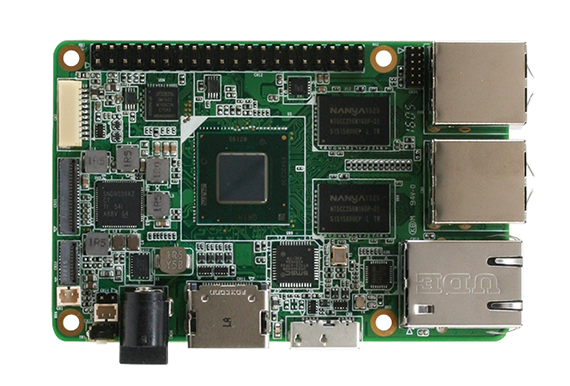
\includegraphics[scale=0.6]{upboard.png}
	\caption{Minikomputer Up Board}
	\label{fig:upboard}
\end{figure}

Platforma posiada jeden port USB 3.0 OGT, przez który jest połączona ze swoim dedykowanym systemem wizyjnym. Liczba dostępnych portów USB 2.0 została zwiększona do siedmiu, poprzez wykorzystanie Qilive Hub. Przy ich pomocy odbywa się komunikacja z lidarem, a także mikro kontrolerem. Moduł wi-fi został wyprowadzony na zewnątrz robota, aby zwiększyć siłę sygnału, ponieważ od niej zależy szybkość przesyłu danych do zdalnego komputera. 

Na platformie został zainstalowany także program RealVNC w trybie serwera. Pozwala on na zdalny dostęp do minikomputera przez wi-fi ze zdalnego komputera, na którym jest zainstalowany pakiet RealVNC w trybie obserwatora. RealVNC na minikomputerze jest uruchamiany przy starcie systemu, dzięki temu zdalny komputer posiada dostęp do \textit{pulpitu} od momentu uruchomienia całego robota. Prędkość transmisji zdalnego obrazu zależy od prędkości sieci na komputerze pokładowym, sprawia to problemy przy słabej jakości połączenia. 

Zasilanie odbywa się z wykorzystaniem przetwornicy napięcia, podłączonej na stałe do wyprowadzeń na płytce. Pozwoliło to na zasilanie platformy z tego samego źródła co napędy. Up Board nie posiada przełącznika odpowiadającego za uruchamianie. Sprawia to, że w momencie podłączenia zasilania uruchamia się samoistnie.
\begin{table}[h]
	\centering
	\caption{Specyfikacja minikomputera Up Board.}
	\label{up_board_specyfikacja}
	\resizebox{\textwidth}{!}{%
		\begin{tabular}{|c|c|}
			\hline
			\multicolumn{2}{|c|}{\textbf{Specyfikacja}}                                                                                                         \\ \hline
			Procesor   & Intel® Atom™ x5-Z8350 Processor (2M Cache, do 1.92 GHz) 64-bitowy,4-rdzeniowy                                                          \\ \hline
			Pamięć RAM & 1GB / 2GB / 4GB DDR3L-1600                                                                                                             \\ \hline
			Dysk eMMC  & 16GB / 32 GB / 64 GB                                                                                                                   \\ \hline
			Grafika    & Intel® HD 400 Graphics                                                                                                                 \\ \hline
			Złącza     & \begin{tabular}[c]{@{}c@{}}4x gniazdo USB 2.0 \\ 2x wyprowadzenie USB 2.0\\ 1x gniazdo USB 3.0 OTG\\ 1x gniazdo HDMI 1.4a\end{tabular} \\ \hline
			Wymiary    & 85.60mm x 56.5mm                                                                                                                       \\ \hline
			Zasilanie  & 5V DC-in                                                                                                                               \\ \hline
		\end{tabular}%
	}
\end{table}

\section{Układ pomiarowy}

Układ pomiarowy służy do mierzenia wybranych wartości fizycznych. Pozwala on na uzyskanie informacji o zachowaniu systemu pod wpływem zadanego sterowania. W budowie robota zostały wykorzystane: system wizyjny, jednostka inercyjna oraz lidar. Wysyłają one informacje na temat otoczenia, a także prędkości i przyśpieszenia robota.
\subsection{System wizyjny}

Wykorzystanym systemem wizyjnym jest dedykowana dla Up Board kamera Intel RealSense R200(Rys. \ref{fig:realsense}).  Najważniejsze dane techniczne zostały przedstawione w Tabeli \ref{kamera}.Dzięki interfejsowi USB 3.0 OTG prędkość przesyłu danych jest wystarczająca na uzyskanie obrazu otoczenia w czasie rzeczywistym. Posiada także bibliotekę umożliwiającą jej komunikację między wątkową ROS.

\begin{figure}[ht]
	\centering
	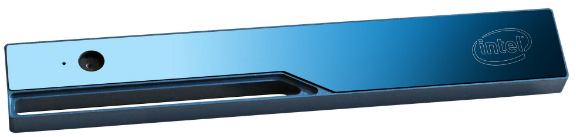
\includegraphics[scale=0.6]{realsense.png}
	\caption{RealSense R200.}
	\label{fig:realsense}
\end{figure}

\begin{table}[]
	\centering
	\caption{Parametry kamery.}
	\label{kamera}
	\begin{tabular}{|c|c|}
		\hline
		\multicolumn{2}{|c|}{\textbf{Specyfikacja}}               \\ \hline
		Zakres pracy                    & 0.5m - 3.5m             \\ \hline
		Rozdzielczość głębokości        & 480 x 360               \\ \hline
		Szybkość w kl/s                 & 60fps                   \\ \hline
		Głębia ostrości i pola widzenia & H: 59, V: 46, D: 70     \\ \hline
		Typ interfejsu systemu          & USB 3.0                 \\ \hline
		Wymiary                         & 101.6mm x 9.6mm x 3.8mm \\ \hline
	\end{tabular}
\end{table}


\subsection{Jednostka inercyjna}

Wykorzystana jednostka inercyjna to MPU-9250(Rys. \ref{fig:imu}), jest to urządzenie 9-osiowe, które wyposażone jest w 3-osiowy żyroskop, 3-osiowy akcelerometr i 3-osiowy magnetometr. Posiada także czujnik temperatury.  Umożliwia komunikację magistralami I2C oraz SPI. W przypadku rozważanego robota wykorzystany został interfejs I2C. Żyroskop informuje o prędkości kątowej robota, pozwala on na ustalenie orientacji. Akcelerometr podaje informacje na temat wypadkowej siły działającej na platformę. W przypadku braku zewnętrznych sił robot jest poddany działaniu tylko siły grawitacji, akcelerometr pozwala się na określenie pozycji platformy względem podłoża. Magnetometr dostarcza informacji na temat ziemskiego pola magnetycznego. MPU-9250 posiada własną bibliotekę Arduino ułatwiającą odczyt danych z czujników.

\begin{figure}[h]
	\centering
	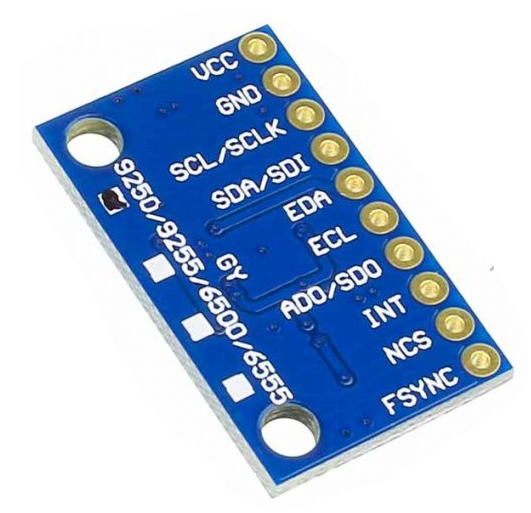
\includegraphics[scale=0.4]{imu.png}
	\caption{Jednostka inercyjna MPU-9250.}
	\label{fig:imu}
\end{figure}

\subsection{Lidar}

Lidar(\textit{Light Detection and Ranging}) jest skanerem laserowym, który pozwala na detekcję elementów otoczenia i poznania odległości od nich. Umożliwia to wykonanie mapy środowiska które jest skanowane przez lidar.

W robocie mobilnym został zamontowany RPLIDAR A1(Rys. \ref{fig:lidar}), jest to  lidar, z możliwością obrotu o 360 stopni. Posiada zasięg do 12m i częstotliwości do 10Hz. Komunikacja następuje przez interfejs UART, połączony z jednostką nadrzędną przez port USB 2.0. Wyposażony jest w dedykowaną bibliotekę do komunikacji między wątkowej ROS.

\begin{figure}[h]
	\centering
	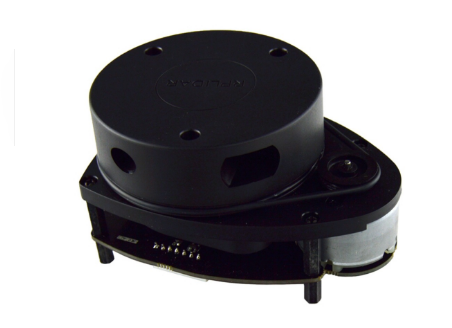
\includegraphics[scale=0.7]{lidar.png}
	\caption{Skaner laserowy RPLIDAR A1.}
	\label{fig:lidar}
\end{figure}



\section{Zasilanie}


Zasilanie konieczne jest dla silników napędowych i platformy Up Board. W tym celu został wykorzystany akumulator litowo-polimerowy Gens Ace 3700mAh 14.8V z serii TATTU(Rys. \ref{fig:lidar}). Jego prąd rozładowania wynosi 45C. Umieszczony jest na zewnątrz robota w celu wygodnego dostępu do ładowania. Połączony jest z układem mocy VNH5019 oraz przetwornicą napięcia w celu obniżenia do 5V, aby możliwe było zasilenie minikomputera Up Board.

\begin{figure}[h]
	\centering
	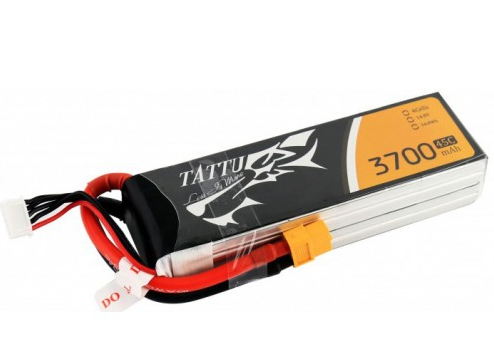
\includegraphics[scale=0.7]{bateria.png}
	\caption{Akumulator z serii TATTU.}
	\label{fig:bateria}
\end{figure}


\chapter{Oprograowanie sterownika silników}

Sterowanie silnikami zrealizowano za pomocą układu mocy VNH5019 połączonego z  STM32 Nucleo-L476RG. Oprogramowanie silników zostało stworzone w języku C oraz z wykorzystaniem bibliotek Arduino. Wiele modułów wykorzystywanych w tworzeniu robota mobilnego posiada gotowe biblioteki Arduino. Mikro kontroler jest kompatybilny z platformą Arduino Uno, pozwala to na uruchomienie programu Arduino na wykorzystywanej platformie STM32.

Do tworzenia oprogramowania użyte zostało środowisko Sloeber, które jest nakładką na zintegrowane środowisko programistyczne Eclipse. Główną zaletą Sloebera jest możliwość tworzenia oprogramowania dla platform Arduino. Środowisko rekomendowane przez producenta Arduino IDE, jest problematyczne w obsłudze w przypadku większych projektów, dlatego do tworzenia oprogramowania został wybrany Sloeber.

Stworzony program, składa się z dwóch głównych funkcji, które są standardem w przypadku programów Arduino. Pierwsza z nich \textit{setup()} odpowiada za inicjalizacje wszystkich wykorzystanych modułów. Drugą z nich jest funkcja \textit{loop()}, która jest  pętlą wykonującą się nieprzerwanie od uruchomienia programu. W niej znajduje się główny program odpowiedzialny za sterowanie i wymianę informacji z jednostką nadrzędną.

\section{Zadawanie i stabilizacja prędkości}

Sterowanie silnikami odbywa się z wykorzystaniem biblioteki od producenta jednostki mocy VNH5019 \textit{DualVNH5019MotorShield.h}. Pozwala ona na sterowanie prędkością kół poprzez zadawanie wartości sygnału PWM(ang. \textit{Pulse-Width Modulation}). 

W celu stabilizacji prędkości zastosowane zostały dwa regulatory PID, po jednym na kanał jednostki mocy.  Składa się on z trzech członów: proporcjonalnego, całkującego i różniczkującego. Ma on na celu utrzymanie prędkości obrotowej kół na zadanym poziomie. Regulator jest on opisany wzorem \ref{fig:PID_ciągły} \cite{pid_continous}.  


\begin{equation}
u(t) = K_p*e(t) + K_i*\int_{0}^{t}e(\tau )d\tau +K_d*\frac{d}{dt}e(t)
\label{fig:PID_ciągły}
\end{equation}
gdzie
\begin{eqwhere}[2cm]
	\item[$e$] uchyb regulacji 
	\item[$K_{p,i,d}$] wzmocnienia członów proporcjonalnego, całkującego i różniczkującego  
\end{eqwhere}

Uchyb regulacji to różnica między wartością zadaną oraz wartością obecną. 
Współczynnik $K_i$ i $K_d$ mogą być także zapisane jako:

\begin{equation}
K_i = K_p * T_i,   K_d = K_p * \frac{1}{T_d}
\label{fig:pid_wzmocnienia}
\end{equation}

gdzie
\begin{eqwhere}[2cm]
	\item[$T_i$] czas całkowania(zdwojenia)  
	\item[$T_d$] czas różniczkowania(wyprzedzenia)  
\end{eqwhere}

Regulator opisany równaniem \ref{fig:PID_ciągły} działa w sposób ciągły. Takie działanie jest niemożliwe do zastosowania w praktyce, ponieważ istnieje tylko skończona liczba pomiarów jakie można wykonać w danej jednostce czasu. W związku z tym zastosowany został dyskretny regulator PID opisany wzorem \ref{fig:PID_dyskretny} \cite{pid_discrete}, w którym okres próbkowania zostaje odgórnie ustalony.

\begin{equation}
u[kh] = K_p*e[kh] + K_i*\sum_{i=0}^{k}e[ih] +K_d*(e[kh]-e[kh-h])
\label{fig:PID_dyskretny}
\end{equation}
gdzie
\begin{eqwhere}[2cm]
	\item[$h$]  okres próbkowania	 
\end{eqwhere}

Okres próbkowania  został ustalony na 10ms. Wyjście z regulatora jest poddane przeskalowaniu do wartości odpowiadającej sygnałowi PWM, a następnie podane jako sterowanie na silniki.


\subsection{Wartość zadana}

Sterownik silników otrzymuje wartość zadaną  od jednostki nadrzędnej. Otrzymana wartość jest w postaci prędkości liniowej i kątowej z jaką ma poruszać się robot. Na podstawie tych prędkości została wyznaczona prędkość z jaką poruszają się prawe i lewe koła robota \cite{wheels_vel}. 

W przypadku poruszania się jednego koła, jego jeden pełen obrót powoduje przesunięcie środka wzdłuż własnej osi o dystans równy \textit{2$\pi$r}, gdzie \textit{r} jest promieniem koła. W przypadku robota posiadającego kilka obrotowych kół, każde koło obraca się wokół własnej osi i muszą one posiadać wspólny środek obrotu(Rys. \ref{fig:diff_drive2}). Ten punkt jest nazywany ICC(\textit{ang. Instantaneous Center of Curvature}). Prędkość każdego koła musi być zgodna ze sztywnym obrotem pojazdu. Oznacza to, że koła nie mogą się poruszać względem siebie.
\begin{figure}[!h]
	\centering
	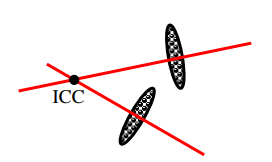
\includegraphics[scale=1]{diff_drive2.png}
	\caption{Dwa obrotowe koła muszą mieć wspólny punkt obrotu.}
	\label{fig:diff_drive2}
\end{figure}

W tworzonym robocie mobilnym koła z lewej i prawej strony poruszają się z tą samą prędkością, w związku z tym model poruszania się został uproszczony do modelu robota dwu kołowego o napędzie różnicowym(Rys. \ref{fig:diff_drive1}). 

Głównym parametrem wyprowadzenia równań kinematycznych jest prędkość kątowa $\omega$, jest zdefiniowana jako obrót każdego koła wokół punktu ICC wzdłuż koła o promieniu \textit{r}.


\begin{figure}[!h]
	\centering
	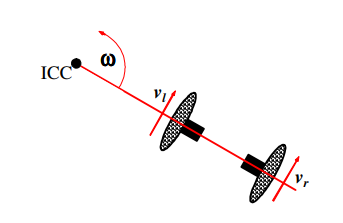
\includegraphics[scale=1]{diff_drive1.png}
	\caption{Konfiguracja kół robota z napędem różnicowym.}
	\label{fig:diff_drive1}
\end{figure}

Prędkość kół jest wyrażona wzorem \textit{v = 2$\pi$r / T} gdzie \textit{T} jest czasem pełnego obrotu wokół punktu ICC. Prędkość kątowa jest zdefiniowana jako \textit{$\omega$ = 2$\pi$ / T} i jest wyrażona w radianach na sekundę. Łącząc równania prędkości \textit{v} i \textit{$\omega$} otrzymujemy równanie \ref{fig:wr=v}.

\begin{equation}
\omega r = v
\label{fig:wr=v}
\end{equation}

Lewe i prawe koła poruszają się z różnymi prędkościami liniowymi oraz po trajektoriach posiadający różny promień, dlatego wyznaczone zostały prędkości liniowe osobne dla koła prawego(\ref{fig:wheel_r}) i lewego(\ref{fig:wheel_l}).
\begin{equation}
\omega (R+\frac{l}{2})=v_r
\label{fig:wheel_r}
\end{equation}
\begin{equation}
\omega (R-\frac{l}{2})=v_l
\label{fig:wheel_l}
\end{equation}
gdzie
\begin{eqwhere}[2cm]
	\item[$R$] odległość punktu ICC od środka robota
	\item[$l$] odległość między kołami 
\end{eqwhere}

Rozwiązując układ równań otrzymano równania opisujące prędkość kątową(\ref{fig:omega}) i promień(\ref{fig:R_rownanie}) układu. Ruch robota został zilustrowany na Rys. \ref{fig:diff_drive3}.

\begin{equation}
\omega = \frac{v_r-v_l}{l}
\label{fig:omega}
\end{equation}
\begin{equation}
R = \frac{l}{2} \frac{v_l+v_r}{v_r-v_l}
\label{fig:R_rownanie}
\end{equation}

\begin{figure}[!h]
	\centering
	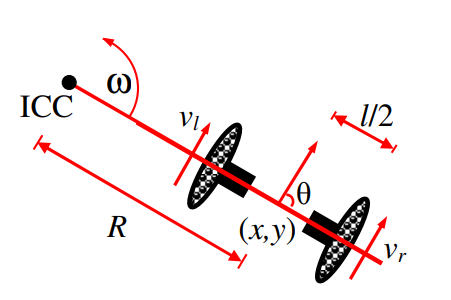
\includegraphics[scale=0.6]{diff_drive3.png}
	\caption{Ruch robota przy różnych prędkościach kół.}
	\label{fig:diff_drive3}
\end{figure}

Podstawiając \textit{$\omega$} i \textit{R} do równania \ref{fig:wr=v} otrzymano prędkość liniową z jaką porusza się robot(\ref{fig:vel_liniowa}).

\begin{equation}
v = \frac{v_l+v_r}{2}
\label{fig:vel_liniowa}
\end{equation}

Następnie wykorzystując równania \ref{fig:omega} i \ref{fig:vel_liniowa} wyznaczono prędkości liniową  prawego(\ref{fig:v_r_finish}) i lewego(\ref{fig:v_l_finish}) koła w zależności od prędkości liniowej i kątowej z jaką porusza się robot.

\begin{equation}
v_r = v + \frac{1}{2}\omega l
\label{fig:v_r_finish}
\end{equation}

\begin{equation}
v_l = v - \frac{1}{2}\omega l
\label{fig:v_l_finish}
\end{equation}

Wyznaczone prędkości liniowe lewego i prawego koła  są wartościami zadanymi regulatorów. Wyrażone są w metrach na sekundę.
\subsection{Wartość pomiarowa}

Wartością zmierzoną wykorzystywaną w regulatorach jest prędkość wyznaczona z wykorzystaniem enkoderów kwadraturowych. Liczniki impulsów zostały zrealizowane przy pomocy przerwań zewnętrznych, które wyzwalane są zboczem narastającym sygnału A(Rys. \ref{fig:encoder_quad}). W momencie wystąpienia impulsu sprawdzany jest stan sygnału B, daje to informację na temat kierunku przesunięcia fazowego sygnałów. Na tej podstawie licznik jest inkrementowany lub dekrementowany.  Enkodery po przeciwnych stronach są zliczane odwrotnie.
\begin{figure}[!h]
	\centering
	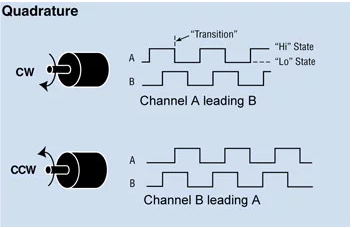
\includegraphics[scale=1]{enkodery.png}
	\caption{Przebieg sygnałów enkodera kwadraturowego \cite{encoder_quad}.}
	\label{fig:encoder_quad}
\end{figure}

Obliczenie prędkości kątowej możliwe jest dzięki wyznaczeniu zmiany kąta obrotu w czasie \cite{encoder_velocity}. Znając liczbę impulsów enkodera na pełen obrót, wyliczono o jaki kąt wykonany został obrót. Przyjęty czas próbkowania wyniósł 5ms. Wyznaczona prędkość kątowa opisana jest wzorem \ref{fig:encoder_omega}. Dysponując prędkością kątową i promieniem koła łatwo wyznaczyć prędkość liniową \ref{fig:encoder_lin}.

\begin{equation}
\omega = \frac{d\Theta}{dt} = \frac{\Delta}{T_s}=\frac{2\pi * \Delta N}{N_p * T_s}
\label{fig:encoder_omega}
\end{equation}

gdzie
\begin{eqwhere}[2cm]
	\item[$N_p$] rozdzielczość enkodera
	\item[$T_s$] czas próbkowania
	\item[$\Delta N$] ilość zliczonych impulsów  
\end{eqwhere}

\begin{equation}
v =\frac{2\pi \Delta N }{N_pT_s}R
\label{fig:encoder_lin}
\end{equation}

Wyznaczone w ten sposób prędkości liniowe poszczególnych kół pełnią role wartości pomiarowej w regulatorach. 
\section{Odometria}
\section{Jednostka inercyjna} 

Jednostka inercyjna MPU9250 posiada dedykowaną od producenta bibliotekę kompatybilną z platformą Arduino. Pozwala ona na inicjalizację komunikacji SPI lub I2C deklarując przy tym odpowiednie piny przystosowane do takich magistrali komunikacyjnych. Funkcja inicjalizacyjna zwraca informację o statusie jednostki, pozwala to na detekcje błędów przed rozpoczęciem odczytów. Biblioteka umożliwia w łatwy sposób odczyt danych z czujników. Posiada możliwość odczytu:
\begin{itemize}
	\item
	\textit{Przyspieszenia liniowego dla 3-osi }
	\item
	\textit{Prędkości liniowej dla 3-osi}
	\item 
	\textit{Orientacji w przestrzeni w postaci kwaterionu}
	\item 
	\textit{Temperatury} 
\end{itemize}
\chapter{Komunikacja między wątkowa w środowisku ROS}

Komunikacja między minikomputerem pokładowym, a zdalnym komputerem została zrealizowana w oparciu o komunikację między wątkową w środowisku ROS. Wykorzystana wersja systemu to ROS Kinetic Kame, która jest kompatybilna z systemem Ubuntu 16.04 Xenial.

Komunikacja przebiega przez sieć wi-fi. W tym celu w pliku \textit{~/.bashrc} zostały zdefiniowane adresy IP wykorzystywane do komunikacji między wątkowej(Tabela \ref{ip_addres}). Umożliwiło to wykorzystanie tego samego rdzenia komunikacji. Węzły odpowiedzialne za generowanie wartości zadanej zostały zainicjalizowane na zdalnym komputerze, natomiast węzły odpowiedzialne za czujniki oraz połączenie z sterownikiem silnika zostały utworzone na minikomputerze pokładowym.



\begin{table}[h]
	\centering
	\caption{Definicja adresów wykorzystywanych przez ROS.}
	\label{ip_addres}
	\resizebox{\textwidth}{!}{%
		\begin{tabular}{c|c|c|}
			\cline{2-3}
			\textbf{}                              & \textbf{Zdalny komputer}             & \textbf{Platforma mobilna}           \\ \hline
			\multicolumn{1}{|c|}{ROS\_MASTER\_URI} & http://IP\_ZDALNEGO\_KOMPUTERA:11311 & http://IP\_ZDALNEGO\_KOMPUTERA:11311 \\ \hline
			\multicolumn{1}{|c|}{ROS\_HOSTNAME}    & IP\_ZDALNEGO\_KOMPUTERA              & IP\_PLATFORMY\_MOBILNEJ              \\ \hline
		\end{tabular}%
	}
\end{table}

\section{Komunikacja jednostki zdalnej}
Rdzeń komunikacji jest inicjalizowany na zdalnej jednostce, ponieważ posiada większą moc obliczeniową. Dodatkowo są na niej uruchamiane węzły odpowiedzialne za zadawanie sterowania, czyli prędkości kątowej i liniowej. Zostało to zrealizowane na trzy sposoby: z wykorzystaniem klawiatury, joysticka oraz MATLABA.

\subsection{Sterowanie w wykorzystaniem klawiatury}

Zadawanie prędkości liniowej i kątowej z wykorzystaniem klawiatury zostało zrealizowane przy pomocy biblioteki \textit{ros-kinetic-teleop-twist-keyboard}. Sterowanie odbywa się poprzez zwiększanie lub zmniejszanie prędkości i wybór, która z prędkości ma być aktywna(Rys. \ref{fig:klawiatura}). Publikowana wiadomość jest w formacie \textit{geometry\_msgs/Twist}, składa się ona z dwóch trójwymiarowych wektorów, jeden z nich odpowiada za prędkość liniową, a drugi za prędkość kątową.

\begin{figure}[ht]
	\centering
	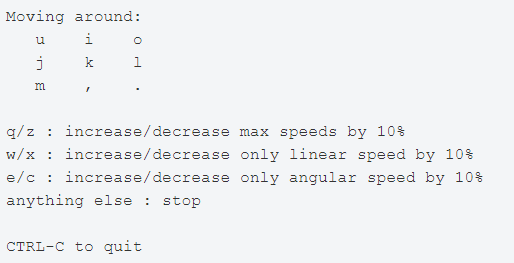
\includegraphics[scale=0.8]{keyboard.png}
	\caption{Sterowanie z wykorzystaniem klawiatury.}
	\label{fig:klawiatura}
\end{figure}

\subsection{Sterowanie z wykrorzystaniem joysticka}
Zostało zrealizowane z wykorzystaniem biblioteki \textit{ros-kinetic-joy}. Wychylenie lewej gałki powoduje zmianę wartości prędkości liniowej i kątowej w zależności od kierunku wychylenia. Wiadomość jest publikowana w formacie \textit{sensor\_msgs/Joy}. Składa się on z wektora określającego poziom wychylenia gałek oraz wektora ze stanem wszystkich dostępnych guzików. Informacja o przyciskach nie jest wykorzystywana, lecz pozwala na rozbudowanie sterowania z wykorzystaniem joysticka o dodatkowe funkcjonalności. 

\subsection{Sterowanie z wykorzystaniem środowiska MATLAB}

Środowisko MATLAB oferuje pakiet \textit{ROS Toolbox}, który pozwala na współprace z system ROS. Zawiera on gotowe funkcje odpowiedzialne za inicjalizację węzła oraz publikowanie i subskrypcję tematu. Dodatkowo obsługuje formaty danych wykorzystywane w komunikacji między wątkowej.  ROS Toolbox posiada także rozszerzenie do Simulink, dzięki któremu dostępne są nowe bloki umożliwiające obsługę ROS.

Sterowanie z wykorzystaniem MATLABa opiera się na stworzeniu węzła w tym środowisku. Program umożliwia stworzenie skryptu, w którym można zadawać sterowanie poprzez publikowanie wiadomości. Wykorzystany format to \textit{geometry\_msgs/Twist}. Takie rozwiązanie posiada przewagę nad dwoma poprzednimi, ponieważ możliwe jest generowanie sterowania na podstawie odczytów z czujników, które węzeł subskrybuje. Pozwala to na stworzenie algorytmów, generujących trajektorię poruszania się robota. Dodatkowo węzeł stworzony w MATLABie pozwala w prosty sposób zmieniać nastawy regulatora wykorzystywanego przez sterownik silników.

\section{Komunikacja jednostki pokładowej}

Minikomputer wbudowany łączy się z rdzeniem uruchomionym na jednostce zdalnej. Odpowiada on za uruchomienie trzech węzłów odpowiadających za system wizyjny, lidar oraz sterownik silników. Węzły są inicjalizowane przy pomocy skryptu napisanego w języku python. 

\subsection{Komunikacja systemu wizyjnego}

Wykorzystanym systemem wizyjnym jest kamera RealSense R200, która jest kompatybilna z minikomputerem pokładowym UpBoard. Komunikacja między wątkowa ROS została przeprowadzona w oparciu o bibliotekę \textit{ros-kinetic-realsense-camera}. Umożliwia ona inicjalizację węzła, który publikuje wiadomości o odczytach z kamery. Wiadomości są publikowane w wielu tematach, odpowiedzialnych za kalibrację, obraz w formacie RGB, głębokość obrazu stworzoną poprzez wykorzystanie dwóch kamer, oraz obraz w podczerwieni. 

\subsection{Komunikacja Lidaru}

Komunikacja z laserowym skanerem została przeprowadzona z wykorzystaniem biblioteki \textit{rplidar\_ros}. Pozwala ona na inicjalizację węzła odpowiedzialnego za lidar. Publikuje on w temacie \textit{scan} wiadomość w formacie 
\textit{sensor\_msgs/LaserScan}. Pozwala to na stworzenie mapy punktów, które zostały zeskanowane przez laser. W połączeniu z jednostką inercyjną lidar umożliwia mapowanie otoczenia robota. 


\subsection{Komunikacja sterownika silnika}

Komunikacja między wątkowa sterownika silnika jest możliwa dzięki bibliotece \textit{roserial}. Pozwala ona na inicjalizację własnego węzła przez wykorzystany miko kontroler STM32. Połączenie odbywa się  z prędkością transmisji wynoszącą 57600 i wykorzystuje port USB \textit{/dev/ttyACM0}.

W oprogramowaniu mikro kontrolera został utworzony węzeł, który pozwala na subskrybowanie tematów i publikację wiadomości.
\subsubsection{Tematy subskrybowane przez sterownik silników}

Subskrypcja tematów pozwala na uzyskanie dostępu do wiadomości, która pojawiła się na obserwowanym temacie. W momencie pojawienia się nowej wiadomości wywołana zostaje funkcja przypisana do danego tematu. Wewnątrz takiej funkcji znajduje się kod programu odpowiedzialny za  przypisanie wiadomości do zmiennych, skąd mogą być wykorzystane w programie. 

Głównymi tematami subskrybowanymi przez sterownik silników są tematy związane z zadawaniem prędkości liniowej i kątowej(Tabela \ref{subscribers}). Dodatkowo subskrybowany jest temat zawierający nastawy regulatora PID, pozwala to w łatwy sposób nimi manipulować.  

% Please add the following required packages to your document preamble:
% \usepackage{graphicx}
\begin{table}[h]
	\centering
	\caption{Tematy subskrybowane przez sterownik silników..}
	\label{subscribers}
	\resizebox{\textwidth}{!}{%
		\begin{tabular}{|c|c|c|}
			\hline
			\textbf{Temat} & \textbf{Opis wiadomości}                                   & \textbf{Format wiadomości}  \\ \hline
			cmd\_vel       & prędkość liniowa i kątowa zadana poprzez konsolę systemową & geometry\_msgs/Twist        \\ \hline
			joy            & prędkość liniowa i kątowa zadana poprzez joystick          & sensor\_msgs/Joy            \\ \hline
			mat\_vel       & prędkość liniowa i kątowa zadana poprzez środowisko MATLAB & geometry\_msgs/Twist        \\ \hline
			pid\_param     & nastawy regulatora PID                                     & std\_msgs/Float32MultiArray \\ \hline
		\end{tabular}%
	}
\end{table}




\subsubsection{Wiadomości publikowane przez sterownik silników }

Sterownik silników publikuje także własne wiadomości na tematy subskrybowane przez zewnętrzne węzły. Podaje on informację o statusie silników, odczytach z czujników, a także wyznaczonej odometri(Tabela. \ref{publishers}). Stworzony został także temat pozwalający na detekcję błędów w oprogramowaniu. Tematy posiadają różną częstotliwość publikowania wiadomości, w zależności od ich zastosowania. 

% Please add the following required packages to your document preamble:
% \usepackage{graphicx}
\begin{table}[h]
	\centering
	\caption{Wiadomości publikowane  przez sterownik silników.}
	\label{publishers}
	\resizebox{\textwidth}{!}{%
		\begin{tabular}{|c|c|c|c|}
			\hline
			\textbf{Temat}    & \textbf{Opis wiadomości}                               & \textbf{Format wiadomości} & Częstotliwość nadawania {[}Hz{]} \\ \hline
			imu               & odczyt z czujników jednostki inercyjnej                & sensor\_msgs::Imu          & 200                              \\ \hline
			odom              & wartości wyznaczonej odometri robota                   & nav\_msgs::Odometry        & 200                              \\ \hline
			imu\_state        & stan jednostki inercyjnej, wartość ujemna oznacza błąd & std\_msgs::Int32           & 30                               \\ \hline
			l\_engines\_state & status silników po lewej stronie, '1' oznacza błąd     & std\_msgs::Bool            & 30                               \\ \hline
			r\_engines\_state & status silników po prawej stronie, '1' oznacza błąd    & std\_msgs::Bool            & 30                               \\ \hline
			debug             & temat służący do debugowania programu sterownika       & geometry\_msgs::Twist      & 30                               \\ \hline
		\end{tabular}%
	}
\end{table}

\chapter{Testy}
testy najlepszego na świecie robota
\section{Test działania sterowania}
no że z matlaba, klawiatury albo padem można pojezdzic
\subsection{Zadawanie prędkości liniowej}
zadanie metr do przodu i ile będzie w rzeczywistości 
\subsection{Zadawanie prędkości kątowej}
zadanie obrót o 360stopni i ile będzie w rzeczywistości
\section{Test działania jednostki inercyjnej}
porównanie prędkości z imu do tej z enkoderów
\section{odometria}
może jakiś obrazek z odometrii, w sensie z rviza jak pojezdził chwilę
\section{Test mapowania pomieszczenia}
raczej bez mapowania i będą tylko punkty z lidaru 
\section{nie wiem co jeszcze}



% itd.
% \appendix
% \include{dodatekA}
% \include{dodatekB}
% itd.

\printbibliography

\end{document}
